%
% File ucca_parsing.tex
%

\documentclass[11pt]{article}
\usepackage{acl2016}
\usepackage{times}
\usepackage{url}
\usepackage{amsmath}
\usepackage{breqn}
\usepackage{latexsym}
\usepackage{pgfplotstable}
\usepackage{algorithm2e}
\usepackage{hhline}
\usepackage{multirow}
\usepackage[font=small]{caption}
\usepackage{subcaption}
\usepackage{hyperref}
\usepackage{color}
\usepackage{lipsum,adjustbox}
\usepackage{tikz}
\usepackage{tikz-dependency}
\usetikzlibrary{shapes,fit,calc,er,positioning,intersections,decorations.shapes,mindmap,trees}
\tikzset{decorate sep/.style 2 args={decorate,decoration={shape backgrounds,shape=circle,
      shape size=#1,shape sep=#2}}}

\newcommand{\oa}[1]{\footnote{\color{red} #1}}
\newcommand{\daniel}[1]{\footnote{\color{blue} #1}}
\newcommand{\com}[1]{}
\newcommand{\secref}[1]{Section~\ref{#1}}
\newcommand{\figref}[1]{Figure~\ref{#1}}
\newcommand{\tabref}[1]{Table~\ref{#1}}
\DeclareMathOperator*{\argmin}{argmin}
\DeclareMathOperator*{\argmax}{argmax}
\SetKwRepeat{Do}{do}{while}
\renewcommand\AlCapFnt{\normalfont\small}

\makeatletter
\renewcommand{\paragraph}{
  \@startsection{paragraph}{4}
  {\z@}{.5ex \@plus .5ex \@minus .2ex}{-1em}
  {\normalfont\normalsize\bfseries}
}
\makeatother

\newcommand\BibTeX{B\textsc{ib}\TeX}

\aclfinalcopy

\title{Supplementary Material}

\begin{document}
\maketitle

\section{$\mathrm{Label}$ function}

\section{Linkage}

\begin{figure}
  \scalebox{.9}{
  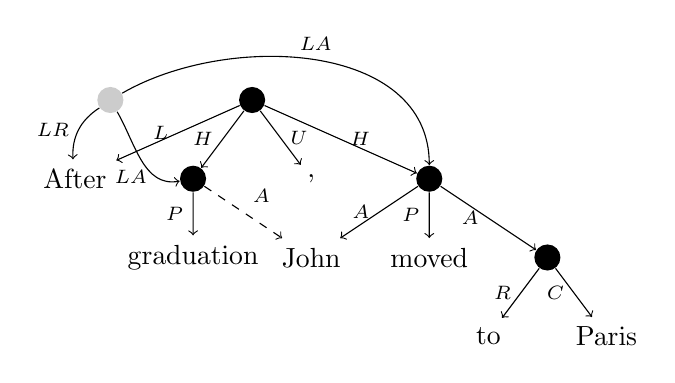
\begin{tikzpicture}[level distance=10mm, ->]
    \node (ROOT) [fill=black, circle] {}
      child {node (After) {After} edge from parent node[left] {\scriptsize $L$}}
      child {node (graduation) [fill=black, circle] {}
      {
        child {node {graduation} edge from parent node[left] {\scriptsize $P$}}
      } edge from parent node[left] {\scriptsize $H$} }
      child {node {,} edge from parent node[right] {\scriptsize $U$}}
      child {node (moved) [fill=black, circle] {}
      {
        child {node (John) {John} edge from parent node[left] {\scriptsize $A$}}
        child {node {moved} edge from parent node[left] {\scriptsize $P$}}
        child {node [fill=black, circle] {}
        {
          child {node {to} edge from parent node[left] {\scriptsize $R$}}
          child {node {Paris} edge from parent node[left] {\scriptsize $C$}}
        } edge from parent node[left] {\scriptsize $A$} }
      } edge from parent node[right] {\scriptsize $H$} }
      ;
    \draw[dashed,->] (graduation) to node [auto] {\scriptsize $A$} (John);
    \node (LKG) at (-1.8,0) [fill=black!20, circle] {};
          \draw[bend right] (LKG) to node [auto, left] {\scriptsize $LR$} (After);
          \draw (LKG) to[out=-60, in=190] node [below] {\scriptsize $LA\quad$} (graduation);
          \draw (LKG) to[out=30, in=90] node [above] {\scriptsize $LA$} (moved);
  \end{tikzpicture}
  }
  \caption{\label{fig:linkage}
}
\end{figure}

\section{Additional example}

The sentence was used by \newcite{oepen2015semeval} to compare between the difference schemes. The sentence includes a single Scene, whose main relation is ``apply'', a secondary relation ``almost impossible'', as well as two complex arguments: ``a similar technique'' and the coordinated argument ``such as cotton, soybeans, and rice.''

\begin{figure*}
\begin{adjustbox}{width=\textwidth}
  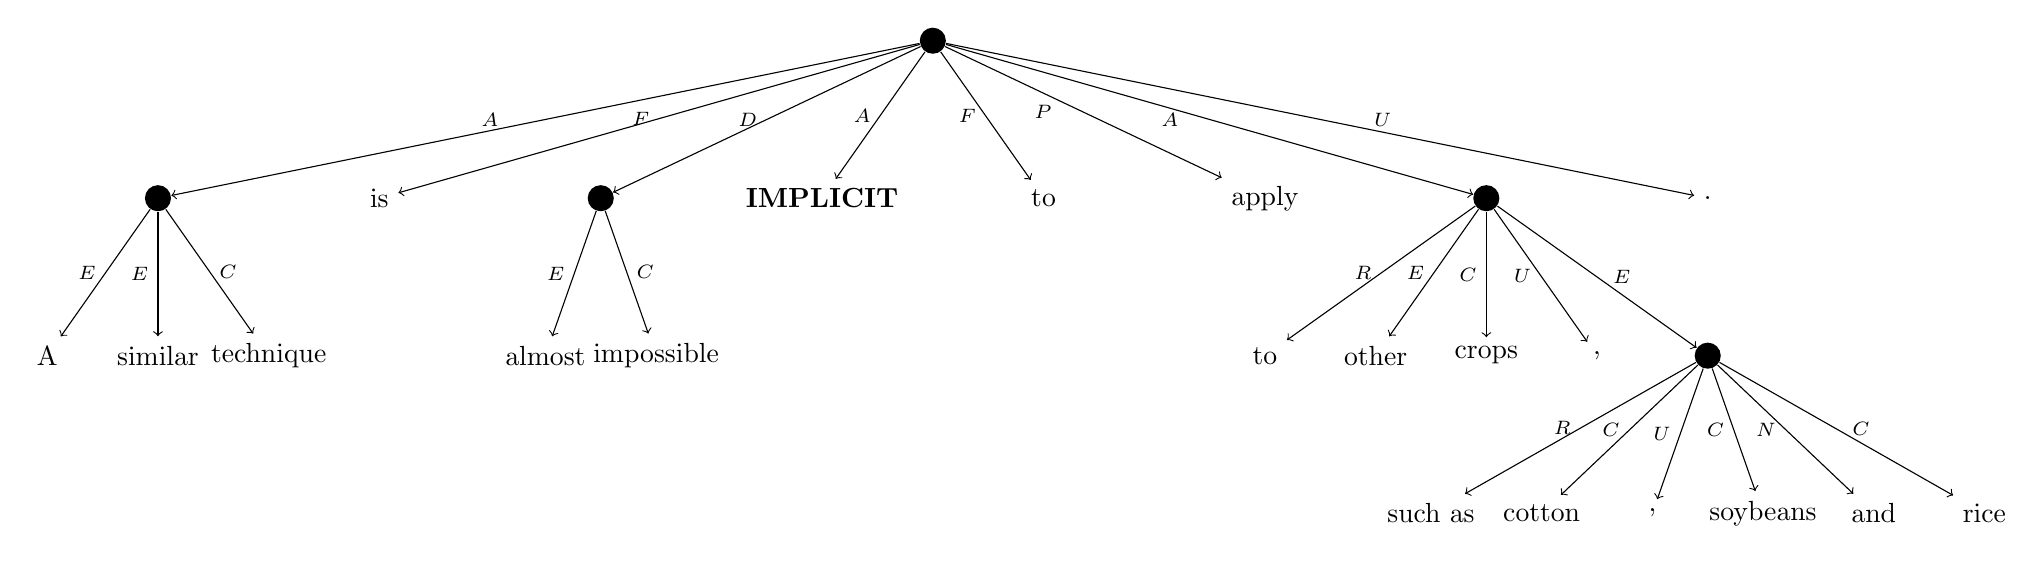
\begin{tikzpicture}[level distance=20mm, ->,
  level 1/.style={sibling distance=8em},
  level 2/.style={sibling distance=4em},
  level 3/.style={sibling distance=4em}]
    \node (ROOT) [fill=black, circle] {}
      child {node [fill=black, circle] {}
      {
        child {node {A} edge from parent node[left] {\scriptsize $E$}}
        child {node {similar} edge from parent node[left] {\scriptsize $E$}}
        child {node {technique} edge from parent node[right] {\scriptsize $C$}}
      } edge from parent node[left] {\scriptsize $A\quad$ \hspace{1mm} } }
      child {node {is} edge from parent node[left] {\scriptsize $F$}}
      child {node [fill=black, circle] {}
      {
        child {node {almost} edge from parent node[left] {\scriptsize $E$}}
        child {node {impossible} edge from parent node[right] {\scriptsize $C$}}
      } edge from parent node[left] {\scriptsize $D$} }
      child {node {\textbf{IMPLICIT}} edge from parent node[left] {\scriptsize $A$}}
      child {node {to} edge from parent node[left] {\scriptsize $F$}}
      child {node {apply} edge from parent node[left] {\scriptsize $P\quad$}}
      child {node [fill=black, circle] {}
      {
        child {node {to} edge from parent node[left] {\scriptsize $R$}}
        child {node {other} edge from parent node[left] {\scriptsize $E$}}
        child {node {crops} edge from parent node[left] {\scriptsize $C$}}
        child {node {,} edge from parent node[left] {\scriptsize $U$}}
        child {node [fill=black, circle] {}
        {
          child {node {such as} edge from parent node[left] {\scriptsize $R$}}
          child {node {cotton} edge from parent node[left] {\scriptsize $C$}}
          child {node {,} edge from parent node[left] {\scriptsize $U$}}
          child {node {soybeans} edge from parent node[left] {\scriptsize $C$}}
          child {node {and} edge from parent node[left] {\scriptsize $N$}}
          child {node {rice} edge from parent node[right] {\scriptsize $\; C$}}
        } edge from parent node[right] {\scriptsize $\; E$ \hspace{1mm} } }
      } edge from parent node[left] {\scriptsize $A\;$ \hspace{1mm} } }
      child {node {.} edge from parent node[right] {\scriptsize $\quad \quad U$}}
      ;
  \end{tikzpicture}
\end{adjustbox}
\caption{\label{fig:ucca_example2}
  UCCA graph for the sentence ``A similar technique is almost impossible to
  apply to other crops, such as cotton, soybeans and rice.''
}
\end{figure*}

\section{Conversion examples}



\bibliography{references}
\bibliographystyle{acl2016}

\end{document}